\documentclass[]{article}

%opening
%\usepackage{fullpage}
\usepackage{hyperref}
\usepackage[english]{babel}
\usepackage[utf8]{inputenc}
\usepackage{graphicx}
%\usepackage[backend=biber]{biblatex}
%\usepackage[]{biblatex}
\usepackage{booktabs}
%\usepackage{amsmath}
%\usepackage{listings}
\graphicspath{{img/}}
\graphicspath{{img/literature/}}
%\usepackage{caption}
%\usepackage{subcaption}
%\bibliography{references}
\title{Biometrics Systems Concepts:\\ 2D + 3D face recognition}
\author{Tom Decroos\\r0297757}
\begin{document}
\maketitle
\begin{abstract}
This report discusses the implementation of a face recognition system that makes use of 2D and 3D face representations. First, two relevant papers are discussed: a paper about using eigenfaces for facial recognition and a paper about using local binary patterns. Next, we describe the implementation of our face recognition system. Our implementation uses methods that are heavily based on the two papers we read. Finally, experiments are performed for 2D face recognition, 3D face recognition and the combination of 2D and 3D face recognition. A recognition rate of 95\% is obtained by applying LBP on all three channels of 2D colour images and fusing them with the $product$ rule.
%TODO

\end{abstract}

\section{Literature study}
We discuss three relevant papers about face recognition systems. The first paper provides a holistic approach for recognizing faces. The used method is eigenfaces. The second paper provides a feature based approach. The used method is local binary patterns.
%The third paper discusses the fusion of 2D and 3D face recognition. It reports on a large experimental study on multimodal face recognition.
For each paper, a small summary is provided. Afterwards, possible advantages and disadvantages of both approaches are discussed. We focus in our summaries and discussion mostly on the parts of the papers that are relevant for this report.

\subsection{Holistic approach: eigenfaces}
The paper we read for recognizing faces with a holistic approach is `Use of depth and colour eigenfaces for face recognition' by F. Tsalakanidou, D.Tzovaras and M.G. Strintzis \cite{tsalakanidou2003use}.
%\paragraph{Summary}
This paper first discusses the extraction of depth maps. Most face recognition systems are based on the evaluation of 2D-intensity or colour im ages. These systems are subject to a variety of errors caused by differences in illumination, head rotation, face pigment or facial expressions. Biometric features from 3D measurements are expected to perform well, due to their relative independence from these differences. One way of exploiting the 3D information of the geometric characteristics of a human face is by building a depth map. The depth map of a face is a function giving for each pixel of an image the distance to the camera. Such a depth map can be extracted from a set of 3D coordinates of points using the z-buffer algorithm.

Next, the classification method is discussed. The paper proposes a powerful global approach (PCA) in which the whole image (colour or depth map) serves as a feature vector and the variability of the face is modelled by analyzing its statistical properties using a large set of faces. PCA is a well-known, widely and successfully used method. The application of PCA for face recognition is very simple: PCA is performed in a well-defined set of images of human faces and a set of principal components is obtained. These principal components are called eigenfaces. Every face in the database can then be represented as a vector of weights. The weights are obtained by projecting the image of the face on the eigenfaces. Identification of a new test image is then done by locating the image in the database whose weights have the smallest euclidean distance from the weights of the test image. The authors of the paper observed experimentally that the accuracy of this approach quickly degrades if there are changes in scale. This can be explained by the low correlation between face images at different scales. Hence, to successfully apply this approach, all faces in the database must be uniformly scaled.

This approach can only be applied on single channel signals such as a depth map or a grayscale image. In case of face recognition from full colour images, this approach is applied to each component of the colour signal. The PCA algorithm is performed for training sets of each component. When a new image needs to be recognized, its projection to the subspace of each component is computed. The image is then assigned to the class that results in the smallest product of the euclidean distances of each component. This combination approach based on the product of the euclidean distances of each component can also be used to combine a colour and a depth map for 2D + 3D face recognition.

Finally, the eigenfaces approach was evaluated on three representations of faces: colour map, depth map and combination of colour and depth. Experiments were performed on images of 40 people. For each person, there were four colour images and two depth maps available. The training set consisted of two colour images and one depth map for each person. The test set consisted of the remaining two colour images and depth map for each person. The eigenfaces approach achieves a recognition rate of 87.5\% using only colour images, 85\% using depth maps and 97.5\% using the combination. These results show that adding depth information leads to significant gains in recognizing faces.

\subsection{Feature based approach: local binary patterns}
The paper we read for recognizing faces with a feature based approach is `Face Recognition with Local Binary Patterns' by T. Ahonen, A. Hadid and M. Pietikäinen \cite{ahonen2004face}.
The paper first explains the concept of local binary patterns (LBP). The original LBP operator is a powerful means of texture description. The operator labels the pixels of an image by thresholding the 3x3 neighbourhood of each pixel with the center value and considering the result as a binary number (Figure \ref{fig:lbp-explained}). This basic operator can be extended by using neighbourhoods of different sizes and using only uniform patterns.
\begin{figure}
\centering
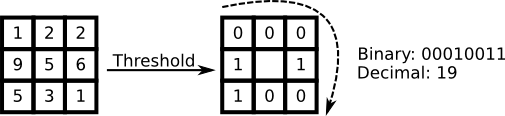
\includegraphics{lbp_explained.png}
\caption{The basic LBP operator.}
\label{fig:lbp-explained}
\end{figure}

The histogram of the labels can then be used as a texture descriptor. This histogram contains information about the distribution of the local micropatterns, such as edges, spots and flat areas, over the whole image. For efficient face representation, one should also retain spatial information. For this purpose, the image is divided into different regions. The histograms of each separate region are then concatenated and form a spatially enhanced histogram. In this histogram, we effectively have a description of the face on three different levels of locality: the labels for the histogram contain information about the patterns on a pixel-level, the labels are summed over a small region to produce information on a regional level and the regional histograms are concatenated to build a global description of the face.

Several possible dissimilarity measures exist for histograms, such as histogram intersection, Log-likelihood statistic and Chi square statistic ($\chi^2$) When the image has been divided into regions, it can be expected that some of the regions contain more useful information than others in terms of distinguishing between people. For example, eyes seem to be an important cue in human face recognition. To take advantage of this, a weight can be set for each region based on the importance of the information it contains. 

The paper used the CSU Face Identification Evaluation System for testing the performance of its proposed algorithm. The results show that $\chi^2$ was the best distance measure between histograms for recognizing faces. They also show that the LBP algorithm is quite robust with respect to its parameters, such as neighbourhood size. Changes in the parameters may cause big differences in the length of the feature vector, but the overall performance is not necessarily affected significantly. When compared to other algorithms such as Eigenfaces, Fisherfaces or Elastic Bunch Graph Matching, the LBP algorithm significantly outperforms them all.

\subsection{Discussion}
Experiments in \cite{chang2005evaluation} suggest that the Eigenfaces approach works best when used on a face space that was generated from a lot of images with diverse conditions (eg. lighting or facial expression). This might be a problem, because our training and test set only consist of five persons each. This means that our face space would be based on only five images. We fear that this face space would incorporate too many specific characteristics of these five images, which would lead to a less accurate result on new images. The LBP algorithm generates features from each image in an independent way, the size of the dataset does not affect its performance. This is a useful characteristic when dealing with small datasets.

It has also been observed experimentally that the performance of the Eigenfaces approach degrades quickly as the scale changes. Intuitively, this is explained by the low correlation between faces and images at different scales. The LBP algorithm considers not only shape, but also texture information to represent face images. That is why we expect the LBP algorithm to be a bit more robust with respect to scale than the Eigenfaces approach.

% eigenfaces need more data
% eigenfaces don't scale well
% sensitive to light
%lbp is independent from other data
%lbp searches for patters, size is less important.
%micro-patterns invariant to monotonic grey scale trasnformation
%\subsection{Fusion of 2D and 3D face recognition}

\section{Methods}
\graphicspath{{img/methods/}}
In this section, we describe our methods for face recognition on 2D colour images and 3D point clouds. We describe the conversion of a colour image in three different channels and the conversion of a point cloud into a depth map. Next, we state our used similarity measure between channels and motivate this choice. We list possible ways of combining similarity measures of different channels. Finally, we explain a preprocessing procedure for 2D images.

\subsection{Channels}
Algorithms such as Eigenfaces or the LBP algorithm require images to be represented as a matrix $X$. The element $x_{ij}$ then represents the value of the pixel at position $(i,j)$. Colour images do not have a single value per pixel, they have three. A colour image can easily be converted into a grayscale image, but then some information about the image is lost. To prevent information loss,  all colour images are split in their three colour channels (Figure \ref{fig:colour-channels}).

\begin{figure}
	\centering
	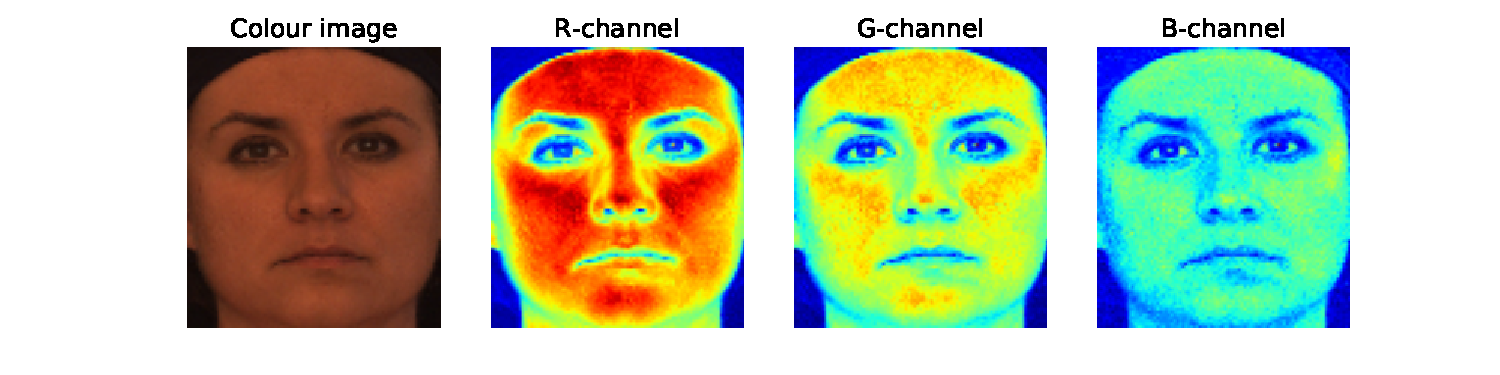
\includegraphics[width=\textwidth]{coloursplitting.pdf}
	\caption{Example of a colour image being split into its three different colour channels}
	\label{fig:colour-channels}
\end{figure}

Converting a 3D point cloud into a 2D matrix that still represents a face is not as trivial however. We convert the point cloud into a depth map. This depth map should show a front view of the face. The value of each pixel in this depth map should represent how close the face was to the camera in the location of that pixel. We construct a depth map in the following way.

We first remove outlier points that definitely do not belong to the face. These outlier points can be detected using statistical measures such as the robust Mahalanobis distance or we can also set arbitrary thresholds based on some exploratory data analysis. All observed faces of the dataset used in this report showed no $x$,$y$ or $z$-coordinates with an absolute value greater than 200, while all outliers always had the same specific coordinate: (999999,999999,999999). Since the 3D point clouds used in this report only contain one specific type of outlier, a threshold that filters these points is deemed good enough to remove all outliers. In our implementation for our given dataset, all data points should satisfy the constraint: $|x|<500 \wedge |y| < 500 \wedge |z| < 500$.

It seems that the 3D point clouds of the faces in our dataset are roughly aligned with the $xy$-surface. This means that a depth map of the face can be constructed by looking only at the $z$-coordinates. To construct a depth map of size $m \times n$, we need the $z$-coordinates of all data points of the intersections on a $m \times n$ grid overlaying the 3D face on the $xy$-surface. Unfortunately our point cloud does not follow a grid-like structure. To solve this, we first overlay the face with the smallest rectangle that still covers all data points. This rectangle is then split in a  $m \times n$ grid. The $z$-coordinates of all points on this grid are then linearly interpolated. In our implementation this linear interpolation is done by first triangulating the point cloud using Qhull and performing linear barycentric interpolation on each triangle \cite{linearinerpolator2016}.
Points on the grid that cannot be interpolated because they fall outside the convex shape of the point cloud are given the same $z$-value as the point with the lowest $z-value$ in the point cloud. These points represent a wall behind the face. Finally, the $x$ and $y$-coordinates of the grid are dropped and only the interpolated $z$-values are kept in a $m \times n$ matrix. Figure \ref{fig:depthmap-generation} illustrates the different steps in the construction of a depth map.
%Finally, the values in the matrix are normalised such that the lowest value is zero.
\begin{figure}
	\centering
	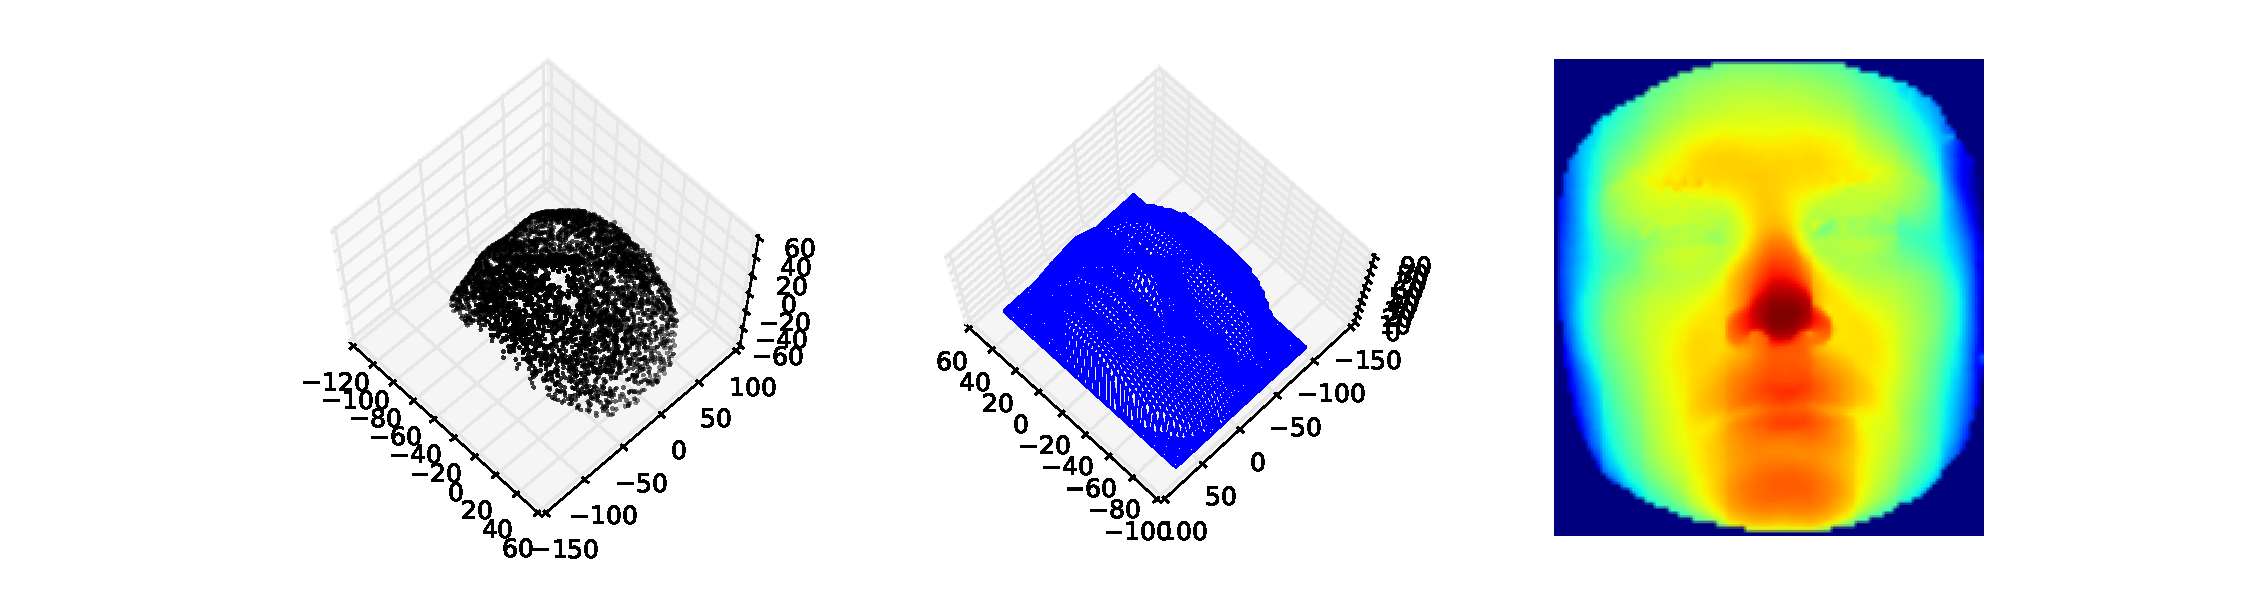
\includegraphics[width=\textwidth]{depthmapgeneration.pdf}
	\caption{Conversion of a 3D point cloud of a face into a depth map by constructing a grid and interpolating the Z-coordinates of that grid.}
	\label{fig:depthmap-generation}
\end{figure}


%splitting colour images in 3 channels
%how depth map was generated, 1.remove outliers 2. grid data

\subsection{Similarity measure}
We use the LBP algorithm to measure the similarity between two faces. We prefer LBP over Eigenfaces for a number of reasons. The original paper that applies LBP to face recognition claims the technique works better than Eigenfaces \cite{ahonen2004face}. We confirmed this on our own dataset through pilot experiments. Furthermore, the quality of the similarity measure is independent from the quality and quantity of the training data, whereas the quality of the Eigenfaces method varies with the training data. This is not a good characteristic when dealing with a small dataset of only 10 people, as in this report. Finally, LBP has the nice property that it is invariant to monotonic grey scale transformations. This means that its recognition rate is barely affected by different lighting conditions.

Each image is converted to a spatial histogram through the following parameters. The used operator is the original LBP operator which labels pixels using their 3x3 neighbourhoods. Each label is thus made up of 8 bits. Each image is divided in a $8 \times 8$ grid of regions. This is a common value used in publications \cite{facerecognizer2016}. The total spatial histogram thus consists of 64 concatenated histograms.

To measure the similarity between histograms, the $\chi^2$ method is used. This is the same similarity measure that is used in the original paper we discussed. It is also a popular and well performing metric for texture comparisons and image retrieval in general \cite{puzicha1997non}.

\subsection{Fusing recognizers}
By using the methods in the previous section, we construct four different face recognizers, one for each channel. Given a probe, these recognizers provide match scores for all persons in the gallery. A match score is the similarity between a given probe and a person in the gallery. The lower the match score, the more likely it is that the probe is the face of that person.

Fusing different recognizers is done by combining the match scores for each person over each channel and predicting the person with the best score. In this report, we try four different fusion rules suggested in a paper by Chang, Bowyer and Flynn \cite{chang2005evaluation}.

%\paragraph{Sum rule}
%For each person, the match scores on all channels are summed. The probe face gets the label of the person with the lowest total match score.
%\paragraph{Product rule}
%For each person, the match scores on all channels are multiplied. The probe face gets the label of the person with the lowest total match score. 
%%	\item[Minimum rule] For each person, the minimum of the match scores on all channels is selected. The probe face gets the label of the person with the lowest minimum match score.
%%	\item[Confidence rule] For each channel, the confidence of that channel is calculated as follows:
%%	\[\frac{distance_2 - distance_1}{distance_3 - distance_1}\] where $distance_i$ is the $i$th smallest distance from the probe to one of the gallery faces. If the difference between the first and second distance metric is large compared to the typical distance, then this value will be large.
%%	The probe face gets the label with the lowest match score from the channel with the highest confidence.
%%\end{enumerate}

\begin{itemize}
	\item \textbf{Sum rule}\\For each person, the match scores on all channels are summed. The probe face gets the label of the person with the lowest total match score.
	\item \textbf{Product rule}\\For each person, the match scores on all channels are multiplied. The probe face gets the label of the person with the lowest total match score. 
	\item \textbf{Minimum rule}\\For each person, the minimum of the match scores on all channels is selected. The probe face gets the label of the person with the lowest minimum match score.
	\item \textbf{Confidence rule}\\ For each channel, the confidence of that channel is calculated as follows:
	\[\frac{distance_2 - distance_1}{distance_3 - distance_1}\] where $distance_i$ is the $i$th smallest distance from the probe to one of the gallery faces. If the difference between the first and second distance metric is large compared to the typical distance, then this value will be large.
	The probe face gets the label with the lowest match score from the channel with the highest confidence.
\end{itemize}

\subsection{Optional: preprocessing 2D images}
The 2D colour images in our given dataset are already of pretty high quality and all have more or less the same format (eg., similar posture, similar distance to camera, similar lighting, etc.). These images can thus be directly fed into our face recognizers. However, we can still perform two normalization steps: a rotation step and a crop step. These two normalization steps could in theory also be applied to more diverse images that have an obtrusive background and/or show more than just the face. Hence, the performance of our recognizers on the preprocessed 2D images should represent the performance on more diverse images than the almost perfect dataset we were given.

Each image in our dataset is accompanied by a landmarks file. This file contains the coordinates of some landmarks on the face. Examples of these landmarks are: middle left eyebrow, inner right eyecorner, nose tip, left mouth corner, chin middle, etcetera. These landmarks are used in both steps of the normalization process.

We first straighten the face by rotating the image such that the eyes are perfectly horizontal aligned. To do this, we calculate the angle between the outer left eye corner and the outer right eye corner. Finally, the figure is rotated to correct this angle using the nose tip landmark as a central point.

Next, the face is cropped by the smallest rectangle that still contains all landmarks. This strategy ensures that all landmark textures are still visible on the cropped figure, while still removing as much of the surrounding figure as possible.

An example of the normalization process (both the rotation and the crop step) is illustrated in Figure \ref{fig:preprocess}.

\begin{figure}
	\centering
	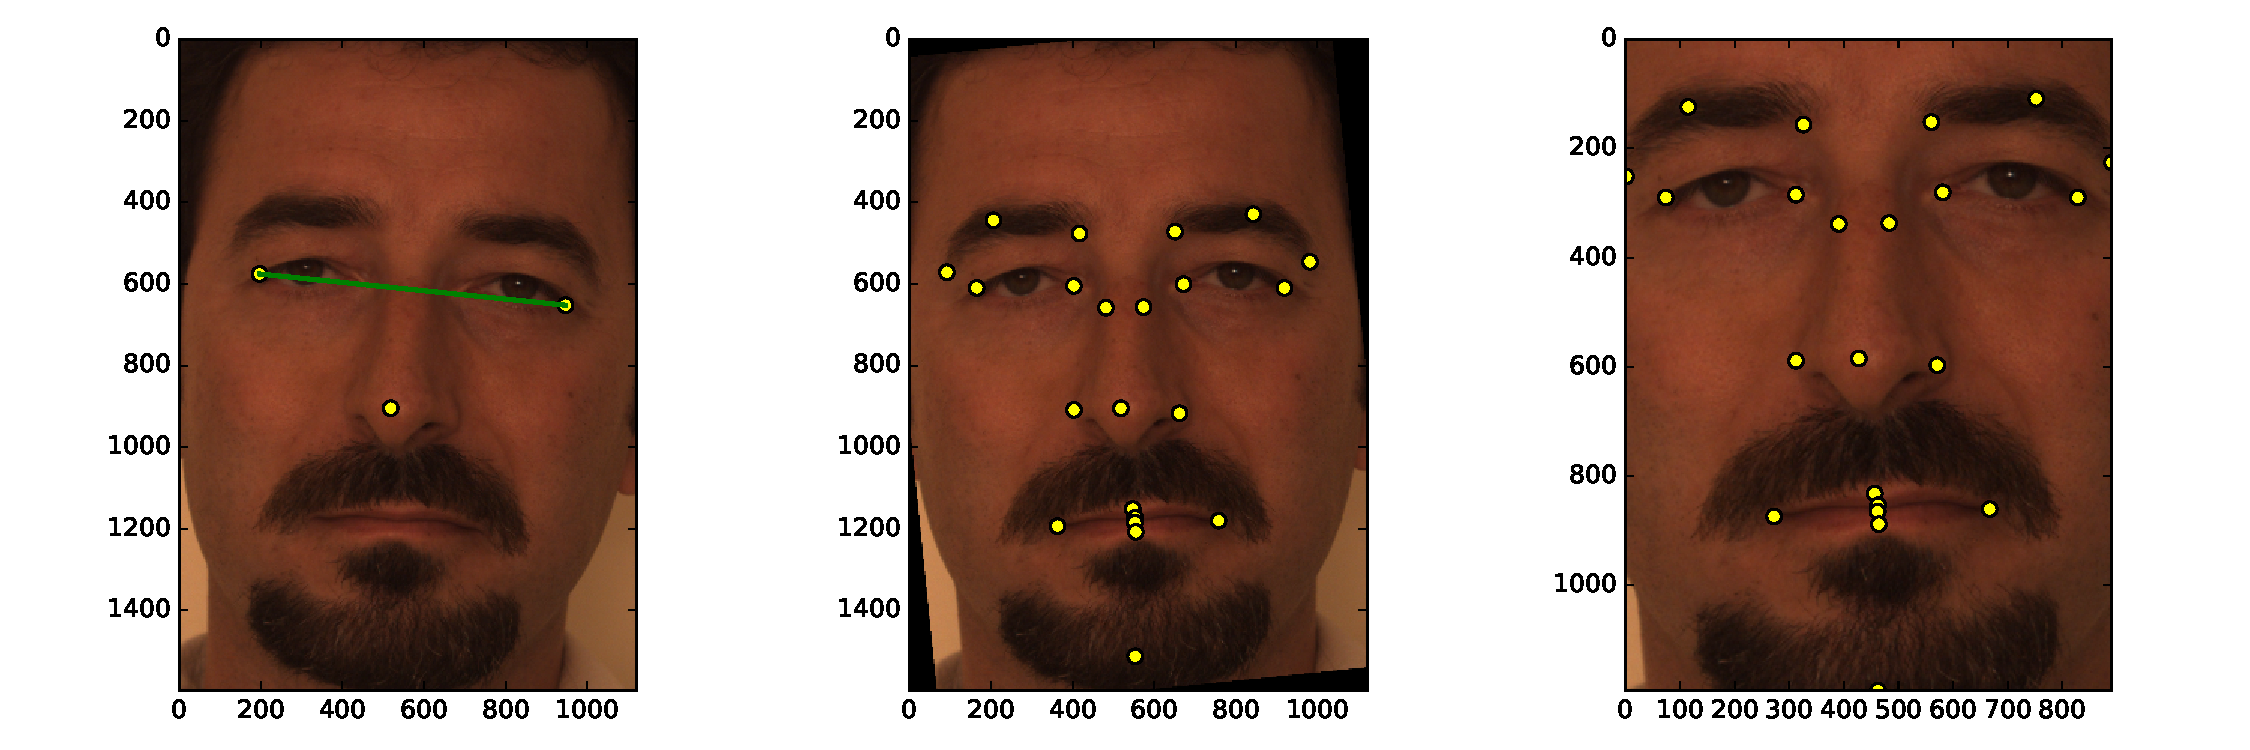
\includegraphics[width=\textwidth]{preprocess2D.pdf}
	\caption{Preprocessing an image by rotating it such that the eyes are horizontally aligned and afterwards cropping it to the smallest possible rectangle such that all landmarks are still contained in the figure.}
	\label{fig:preprocess}
\end{figure}

\section{Experiments}
\graphicspath{{img/experiments/}}
We have conducted experiments to attempt to answer the following research questions.
\begin{itemize}
	\item[Q1] Which performs better: 2D or 3D face recognition?
	\item[Q2] Does fusion significantly raise the recognition rat? If so, what is the best way to fuse match scores?
	\item[Q3] Is it better to preprocess the 2D face images or do the raw images perform better?
\end{itemize}

We have implemented our face recognition system in Python. All experiments were run on a laptop running Windows 8.1 with an Intel Core i5-4210U CPU running at 1.7GHz and 4GB of RAM. All images were resized to a width of 135 pixels and a height of 150 pixels after any necessary preprocessing steps and just before being fed to the LBP face recognition algorithm.

The dataset used in our experiments is a subset of the Bosphorus database and contains 2D and 3D images of 10 subjects. The assignment for this report stated that the first 5 subjects could be used for training and the last 5 subjects were to be used for testing. The assignment further stated that the neutral faces were to be used as gallery images and all other images as probe images.

\begin{table}
	\centering
	\begin{tabular}{lrrr}
		\toprule
		& training set & test set & all faces\\
		\midrule
		R-channel (2D) & 0.968 & 0.867 & 0.902\\
		G-channel (2D) & 1 & 0.8 & 0.885 \\
		B-channel (2D) & 1 & 0.63 & 0.803 \\
		Depthmap (3D) & 0.548 & 0.7 & 0.607 \\
		\bottomrule
	\end{tabular}
	\caption{Recognition rates for different combinations of channels and sets of subjects.}
	\label{tab:traintestall}
\end{table}

\paragraph{Q1} Table \ref{tab:traintestall} shows the recognition rate for each separate channel for the training set, the test set and all subjects. The 2D channels clearly show better performance than the 3D channel. This conflicts with observations in \cite{chang2005evaluation,tsalakanidou2003use} which state that similar recognition rates can be obtained using a single 2D image or a single 3D image. This suggests that our implementation of a 3D face recognition might be subpar. A possible improvement to our system could be to first properly align all faces in 3D space, before constructing a depth map. Our current system does not do this and assumes that all 3D faces are already aligned with the xy-surface. This assumption was based on an exploratory data analysis, but might not hold for the entire dataset.

We note that the recognition rate between the training set and the test set varies greatly. This means that the performance of our face recognition system on the training set is not an accurate estimator of the performance on the test set. Furthermore, we already achieve a perfect recognition rate for some channels on the training set. The performance of our face recognition system can thus not be improved when tuning purely on the training set. Splitting a dataset in a training set and a test set is usually done to prevent the overfitting of parameters when tuning a classification system. However, this is only advised when there is enough data available. Since we only have 10 subjects and do not perform any rigorous parameter tuning, we choose to test different configurations of our face recognition system on the entire dataset for the remainder of our experiments.

\begin{table}
	\centering
	\begin{tabular}{lrrrr}
		\toprule
		& Sum & Product & Minimum & Confidence\\
		\midrule
		Colour (2D) & 0.951 & 0.951 & 0.803 & 0.836\\
		Colour and Depth (2D + 3D) & 0.738 & 0.770 & 0.803 & 0.803 \\
		\bottomrule
	\end{tabular}
	\caption{Recognition rates of the entire dataset of fused face recognition systems for different fusion rules.}
	\label{tab:fusion-rules}
\end{table}

\paragraph{Q2} We evaluate two fused face recognition system. The first face recognition systems combines the three colour channels. The second face recognition system adds depth to the mix and thus combines all four channels. Table \ref{tab:fusion-rules} shows the recognition rates of these two face recognition systems for different fusion rules. We can see that fusion has a positive effect. A higher recognition rate is achieved when all three colour channels are combined than for any single channel. The fusion of 2D and 3D actually lowers the recognition rate, compared to just 2D alone. This happens most likely due to the bad performance of our 3D face recognition system.

Fusion rules that combine all match scores such as $Sum$ and $Product$ achieve a high recognition rate when combining channels of high quality (ie., the 2D channels), but show a drop in performance when combined with a channel of lesser quality (the 3D channel). Fusion rules that select the best channel based on some criterium ($Min$ and $Confidence$) do not achieve better performance than their individual parts, but do appear to be a bit more robust when combined with a channel of lesser quality. Our recommendation is thus to use the $Product$ rule when it is known that all channels show similar good performance and to use the $Confidence$ rule when it is not sure that all channel are reliable.

\begin{table}
	\centering
	\begin{tabular}{lrr}
		\toprule
			& raw & preprocessed\\
		\midrule
		R-channel (2D) & 0.902& 0.902\\
		G-channel (2D) & 0.885& 0.869 \\
		B-channel (2D) & 0.803& 0.754  \\
		Colour (2D) & 0.951& 0.934\\
		Colour and Depth (2D + 3D) & 0.770 & 0.820\\
		\bottomrule
	\end{tabular}
	\caption{Recognition rates for different face recognition systems using either raw or preprocessed 2D images. The fused recognition systems used the $Product$ fusion rule.}
	\label{tab:preprocess-rr}
\end{table}

\paragraph{Q3}
Table \ref{tab:preprocess-rr} shows the recognition rates for different face recognition systems using either raw or preprocessed 2D images. No significant drop or increase in performance is detected. We definitely did not expect a huge increase in performance, since the images in our given data are already of high quality and have very similar formats. The fact that similar recognition rates are achieved on the preprocessed images suggest that almost no useful information and/or characteristics of the face are lost during the processing steps. We therefore believe that our face recognition system for 2D images could be successfully applied to more diverse images, as long as they contain a front view of the face of the person to be recognized.

\section{Conclusion}
This report discussed our implementation of a face recognition system that makes use of 2D and 3D face images. Two relevant papers for recognizing faces were discussed. The first paper described a holistic approach: Eigenfaces. The second paper introduced a feature based approach: local binary patterns (LBP). We split 2D images up in three colour channels and convert a 3D point clouds into depth maps by interpolating values on a 2D grid. We chose to use LBP as our distance measure, because it had a couple of clear advantages over Eigenfaces, such as being shown to perform better in its introductory paper and being independent from the quality and quantity of data in the training set. We listed four different fusion rules. We described our approach for preprocessing 2D face images through a rotation and crop step based on the accompanying anatomical landmarks.

Experiments suggest that our implementation of a 3D face recognition system is subpar compared to other work. Fusion of recognition systems increases the recognition rate. The best rule for fusing face recognition systems is the $Product$ rule if all individual face recognition systems show good performance. Otherwise, the $Confidence$ rule appears to be the most robust. Preprocessing faces shows no significant increase or decrease compared to the raw images. This leads us to believe that our face recognition system would also perform well on more diverse images. A recognition rate of 95\% is obtained by applying LBP on all three channels of 2D colour images and fusing them with the $product$ rule.
\bibliography{references}
\bibliographystyle{IEEEtran}
\end{document}